\documentclass[a4paper,12pt,notitlepage]{article}
\usepackage[T2A]{fontenc}
\usepackage[utf8]{inputenc}
\usepackage[russian]{babel}
\usepackage{fullpage}
\usepackage{color}
\usepackage[table]{xcolor}
\usepackage{etoolbox}
\usepackage{mathtools}
\usepackage{multicol}
\usepackage{verse}
\usepackage{hyperref}
\usepackage{minted}

\setlength{\parskip}{0.7em}

\hypersetup{
    pdftitle={Alter Mann},
    colorlinks=true,
    linkcolor=blue,
    citecolor=blue,
    filecolor=magenta,      
    urlcolor=cyan,
}

\author{Дмитрий Григорьев}
\title{Граф взаимоотношений персонажей\\песни <<Alter Mann>> группы Knorkator}

\renewcommand{\listingscaption}{Листинг}
\renewcommand{\listoflistingscaption}{Список листингов}

\begin{document}
  \maketitle

  В 2007 году популярный немецкий музыкальный коллектив Knorkator выпустил на лейбле Nuclear Blast свой шестой альбом <<Das Nächste Album Aller Zeiten>>. Первой песней в альбоме стала песня <<Alter Mann>> (<<Старик>>).
	
	\begin{figure}[ht]
    \centering
    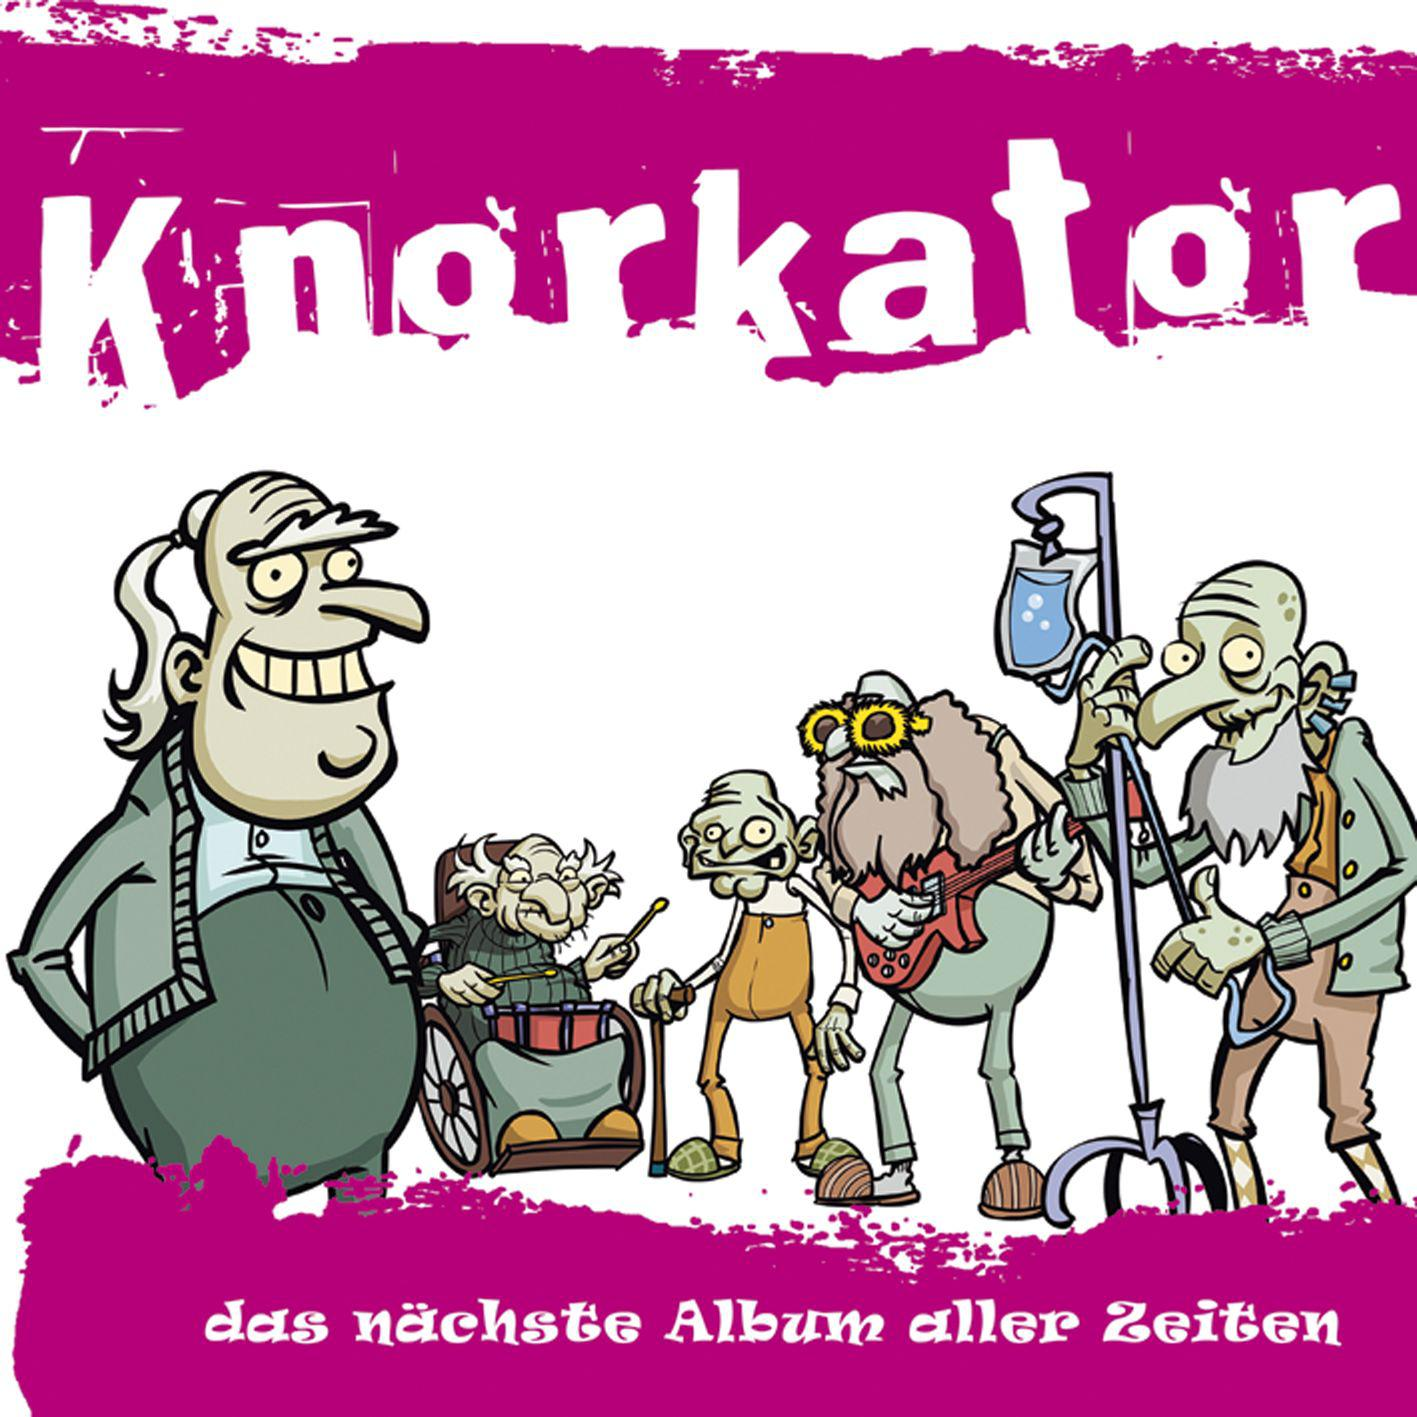
\includegraphics[width=8cm]{coverart.jpg}
    \caption{Обложка альбома <<Das Nächste Album Aller Zeiten>> группы Knorkator}
    \label{fig:graph}
  \end{figure}

  В песне представлены сложные взаимоотношения различных персонажей и демонстративно индифферентное отношение лирического героя песни (<<Старика>>) к ним (одновременно с нескрываемым желанием всё же наблюдать за ними). Текст песни на немецком языке \cite{knorkator01}:
  
	\newpage

  \poemtitle{Alter Mann}
  
  \settowidth{\versewidth}{Doch Pech denn er ist schon länger}

  \begin{verse}[\versewidth]
	  \flagverse{1.}Daniela steht auf Jonas, \\*
	  Doch Jonas liebt Vanessa, \\*
		Vanessa wär gern mit Lars zusammen, \\*
		Doch der findet Melanie besser. \\*
		Die allerdings steht eher auf Tim, \\*
		Tim wiederum findet Jennifer cool, \\*
		Jennifer jedoch ist verliebt in Kevin, \\*
		Aber Kevin ist schwul. \\!
		Tobias ist scharf auf Annika, \\*
		Und Annika eigentlich auch auf ihn, \\*
		Doch Pech denn er ist schon länger \\*
		der Schwarm ihrer besten Freundin. \\!

		\flagverse{\textsc{припев}}Zum Glück bin ich ein alter Mann, \\*
		Das geht mich alles nichts mehr an, \\*
		Bin weder Hetero noch schwul, \\*
		Und mir genügt ein angenehmer Stuhl. \\!

		\flagverse{2.}Hagen erschießt Sebastian, \\*
		Sven überfährt Hagen, \\*
		Christopher erwürgt Sven \\*
		Und wird von Yannick erschlagen. \\*
		Björn und Jochen ermorden Yannick, \\*
		Lukas erledigt Björn und Jochen, \\*
		Benjamin macht Lukas alle, \\*
		Und wird von Nils erstochen. \\!
		Nils wird daraufhin abgemurkst, \\*
		Von Felix und Thorsten, \\*
		Alexander killt Thorsten und Felix, \\*
		Und wird erschossen. \\!

		\flagverse{\textsc{припев}}Zum Glück bin ich ein alter Mann, \\*
		Das geht mich alles nichts mehr an, \\*
		Auf dem Balkon hab ich es gut, \\*
		Und schau was ihr da unten alles tut. \\!

		\flagverse{\textsc{бридж}}Ich hab eh nicht mehr lange, \\*
		In diesem irdischen Jammertal, \\*
		Schlagt doch alles in Stücke, \\*
		Es ist mir so egal. \\!
		
		\flagverse{\textsc{припев}}Zum Glück bin ich ein alter Mann, \\*
		Das geht mich alles nichts mehr an, \\*
		Und wenn die Erde explodiert, \\*
		Entschuldigt dass es mich nicht interessiert. \\*
		Entschuldigt dass es mich nicht interessiert! \\
  \end{verse}
  
  В первом куплете описаны любовные отношения ряда персонажей различного сорта и успешности, во втором куплете --- вражда, сопровождаемая насилием и убийствами. Весь остальной текст выражает отношение к происходящему лирического героя. После внимательного прослушивания песни и анализа текста, мы можем построить следующий социальный граф в формате \texttt{dot}: (\ref{lst:dot}).

	Мы также указываем детали оформления визуализации графа. Персонажи первых двух куплетов объединены в подграфы, каждый из которых имеет собственную рамку. Неявно указанные отношения персонажа Kevin (о нём говорится, что он schwul, т.е. потенциально может иметь романтическую связь с любым из персонажей-мужчин) представлены пунктирной линией.
  
  \begin{listing}[H]
    \caption{Graphviz-файл \texttt{altermann.dot}}
    \label{lst:dot}
    \inputminted[linenos,fontsize=\small]{dot}{altermann.dot}
  \end{listing}
    
  \newpage

  В результате обработки исходного кода графа программой \texttt{dot}, входящей в пакет \href{https://http://www.graphviz.org/}{Graphviz}, после выполнения команды \mint{bash}|dot -Tpng altermann.dot > altermann.png| получаем изображение \ref{fig:graph}.
    
  \begin{figure}[ht]
    \centering
    \includegraphics[width=8cm]{altermann.png}
    \caption{Социальный граф, построенный по тексту песни <<Alter Mann>>}
    \label{fig:graph}
  \end{figure}
    
  \newpage

  \listoflistings

  \listoffigures

  \begin{thebibliography}{1}
    \bibitem{knorkator01}
    Knorkator --- <<Alter Mann>>, (\href{https://genius.com/Knorkator-alter-mann-lyrics}{genius.com}), Das nächste Album aller Zeiten, NB 1779-0, 2007
  \end{thebibliography}
      
\end{document}